
%% Introduction

Virtual reality combines real-time computer graphics, body-tracking devices and high-resolution visual displays to create a computer-generated virtual environment. With their ability to immerse the user into a virtual mirror of the real world, virtual environments are a powerful tool in clinical application, especially in the treatment of phobias (Riva, 2003). \\
Studies have shown anxiety disorders to be the most prevalent mental disorders (Kessler et al., 2005). Many consider exposure therapy the most effective form of treatment for specific phobias (DeRubeis and Crits-Cristoph,1998). However that may be, considering the nature of certain phobias such as fear of heights, exposure therapy involves a genuine risk of injury. Performing therapy in a virtual environment therefore can be a promising alternative to the conventional in-vivo exposure.\\ 
The efficacy of virtual reality exposure therapy (VRET) has already been demonstrated in the past. A study conducted on acrophobia compared two groups of student subjects. The first group received a graded VRET. Students of the second group were added to a waiting-list as a control group. Results showed that VRET is more effective than no treatment (Rothbaum et al.,1995). VRET was also found to be as effective as exposure in-vivo in a more recent work by Emmelkamp et al. (2002).\\
In addition to this using a virtual reality system can have a number of advantages over in-vivo exposure. First and foremost being the ability to conduct therapy inside a controlled and secure environment like a therapist's office. This also implies therapy being less time consuming and provides considerable financial benefits (Cavanagh and Shapiro, 2004). The possibility of having therapy in a more private scenario also could lead to it becoming a more attractive choice for patients, that are too anxious or fear public embarrassment. 
A recent study exploring the acceptability of virtual reality exposure and in-vivo exposure in subjects suffering from specific phobias supports this hypothesis. Seventy-six percent chose virtual reality over in-vivo exposure. In addition to this the refusal rate of 3\% for virtual reality exposure was substantially lower than 27\% for in-vivo exposure (Garcia-Palacios et al., 2007). Further epidemiological studies show a lifetime prevalence of 28.5\% for vHI and 6.4\% for acrophobia alone and only 11\% of susceptible people consulting a doctor (Huppert et al., 2013; Kapfhammer et al.,2015).\\
These results suggest that virtual reality exposure could help increase the number of people who seek therapy for phobias and therefore needs to be established in everyday clinical work.\\
In recent years there has been a lot of research on virtual reality treatment for different phobias trying just that.\\
For example a controlled study by Rothbaum et al. on aerophobia (2000) as well as a open clinical trial post-traumatic stress disorder (2001) and a study on agoraphobia (Meyerbröker et al.,2011), all of which yielded positive results.
There also have been studies on ways to control the virtual reality. In a pilot study, Levy et al. (2015) explored the possibility of a remote-controlled virtual reality. After a trial session in a neutral virtual environment the patients received a total of six therapy sessions. The first three sessions were remote-controlled virtual reality exposure therapy (e-VRET) followed by three sessions in the presence of a therapist (p-VRET). E-VRET sessions were conducted without any contact to the hospital staff. The study showed that e-VRET not only is possible but produces results equal to p-VRET. %This inevitably leads us to the idea of a entirely independent VRET. 
%To our knowledge there has not yet been any research on a form of VRET, that does not depend on external control by a therapist. A system, that is able to adapt to the mental state of the patient throughout the entirety of therapy and therefore qualify for private use.  This could help expanding the reach of exposure therapy even further.\\
Assessing the mental state of a patient is essential for the success of the therapy. A task which usually falls to the hands of the therapist and in most cases relies on a verbal communication between both parties.
%To ensure the quality of our therapy system we clearly have to provide some sort of substitute for this.\\
Past studies have shown a strong psychophysiological arousal in in-vivo exposure for different specific phobias (Nesse et al.,1985; Alpers and Sell,2007). In a more recent work Diemer et al. (2015) also confirmed physiological arousal in subjects executing a virtual height challenge. The study examined phobics and healthy controls in terms of subjective and physiological fear reactions resulting in a significant increase of subjective fear, heart rate and skin conductance level. 
%We base our hypothesis on these results and claim a independent virtual reality system, that is able to react according to changes in heart rate and electrodermal activity, is possible.\\
%The present thesis is prior to a study in cooperation with the psychiatry department of the University Clinic Saarland concerning VRET on acrophobia.
%Our goal is to prove that a closed loop virtual reality system able to operate on its own by relying only on real-time physiological data is possible. 
To prove this hypothesis, we designed a virtual environment for the treatment of acrophobia that is sufficiently adaptable to various degrees of acrophobia. We will show the effectiveness of our system based on a subjective rating as well as heart rate and skin conductance measurements. Further we will deploy our virtual environment in a closed loop virtual reality system, featuring multiple control units. We will conduct a experiment simulating the effect of real-time physiology based decision making by using a remote-controlled virtual reality.\\







%%%%%%%%%%%%%%%%%%%%%%%%%%%%%%%%%%%%%%%%%%%%%%%%%%%%%%%%%%%%%%%%%%%%%%%%%%%%%%%%%%%%%%%%



%Suffering from a specific phobia such as acrophobia can be a huge interference with daily life. Those affected are often experiencing a slow progressing self-limitation fueled by their fear resulting in a declining quality of life. For people afflicted with acrophobia a therapy can therefor be life-changing.\\
%Typically a therapy is designed to help patients face their fears and practice coping strategies resulting in reducing the fear altogether. However, conducting a traditional exposure therapy can be particularly risky for the patient.
%Virtual reality guided exposure therapy offers the possibility to treat patients in a controlled environment and eliminate the risk of injury. Furthermore virtual reality assisted treatment represents a safer and cost-efficient alternative that has great potential in improving phobia treatment based on its flexibility.\\
%For example a in-vivo therapy consists of many different steps based on the initial extent of a patients fear and requires just as many individual stimulating situations. On the contrary one well designed virtual setup can easily adapt to all therapy stages and therefor be more convenient.\\

\section{Theoretical Background}

In this chapter, we will give a brief introduction to the field of anxiety disorders, especially specific phobias and the associated therapy concept, which is exposure therapy. The first part will contain fundamentals on phobias, exposure therapy and the concept of fear. Furthermore we will elaborate on the psychophysiological influences of stress and anxiety on certain parts of the human body and functions as well as methods of determination in physiological measurement. The second part will recapitulate recent approaches on virtual reality exposure therapy and analyze existing problems. 

\subsection{Acrophobia} 
%definition of fear and specific phobias,prevalence, evolutionary 	 purpose(fight or flight),connection fear to stress
%Vertigo and nausea are only two of the symptoms many people are all too familiar with when confronted with height. Acrophobia or fear of heights is one of the most common anxiety disorders and is widespread in today's society.
%According to the work of Kapfhammer et al. (2014) roughly one third of the German population will at one point in their life be afflicted by visual height intolerance (vHI). Although  considering such high numbers it comes as a surprise that only about 11\% of susceptible individuals are willing to consult a doctor(Kapfhammer et al. 2014).
%Epidemiological research showing a peak in incidence around the second decade ( Huppert et al. 2012, Agras et al. 1969) and  

 
\subsection{Stress}
%definition of stress, ways of stress perception (eustress and distress)

\subsection{Electrodermal Activity}
%%short explanation, influences(autonomic nervous system), role as method  to register physiological correlates of mental states like stress\\
%%
%%- illustration of a typical gsr signal and explanation of its components (graph, peaks etc.) \\
%%
%%- how and where is gsr usually measured? why there?\\
%

%%- exosomatic method of recording skin conductance level and skin conductance response as method of choice ( Fowles et al. 1981)

%%- secretory theory, by tarchanoff relates EDA to sweat gland activity, supported through Darrow 1927 who showed a close relation of the sweat secretion and EDA
%%-scr begins about 1 s earlier than moisture would appear on the skin surface -> gland activity not sweat on the skin itself is critical for EDA
%%- palmar sweat glands are innervated by the sympathetic chain of the autonomic nervous system -> EDA reflects sympathetic activation
%%- In fact, we would date the beginning of
%%the modern era of EDA research to the early 1970s when
%%Lykken and Venables proposed standardized techniques
%%of recording skin conductance and standardized units of
%%measurement
%%- Another issue of central importance concerns the psychological
%%significance of EDA. From the beginning, this
%%response system has been closely linked with the psychological
%%concepts of emotion, arousal, and attention.
%%-“Every stimulus accompanied by an emotion produced
%%a deviation of the galvanometer to a degree in direct
%%proportion to the liveliness and actuality of the emotion
%%aroused” (Peterson, 1907, cited by Neumann & Blanton,
%%1970, p. 470)
%%- Woodworth and Schlosberg ,1954: They supported this indexing relationship by noting that tonic SCL is generally low during sleep and
%%high in activated states such as rage or mental work. The
%%authors also related phasic SCRs to attention, noting that
%%such responses are sensitive to stimulus novelty, intensity,
%%and significance.
%%- Anatomical and physiological basis:
%%- There are two forms of sweat glands in the human
%%body: the apocrine, which have been less studied, and
%%the eccrine, which have been of primary interest to psychophysiologists.
%%The primary function of most eccrine
%%sweat glands is thermoregulation. However, those located
%%on the palmar and plantar surfaces are thought to be more
%%related to grasping behavior than to evaporative cooling
%%(Edelberg, 1972a) and they have been suggested to be more
%%responsive to psychologically significant stimuli than to
%%thermal stimuli.\\

Electrodermal activity (EDA) is a collective term for all electrical phenomena in the skin, which was first introduced by Johnson and Lubin (1966). This includes active and passive electrical properties, caused by skin functions and skin structure as well as the appendages of the skin.%(Thom and Boucsein, 2013). 
The skin appendages are structures formed by skin-derived cells such as hair, nails, sebaceous glands and sweat glands. EDA is one of the most commonly used response systems in psychophysiological research. This is due to its relative ease of measurement and its sensitivity to psychophysiological states and processes. The following section will provide a brief overview of EDA, ranging from physical and psychological context to recording and quantification methods.

\subsubsection*{Anatomical basis} 
This section will elaborate on the anatomical aspects of the human skin and will cover all the parts and appendages, that are needed to understand the principles of EDA. The skin or cutis is the biggest organ of the human body and inherits many different functions, which are essential for survival. It primarily acts as a selective barrier, preventing the entry of foreign matter and enables the passage of materials from the bloodstream to the exterior of the body. Other than protection, it is involved in thermoregulation, cutaneous circulation and immunologic protection.  
The anatomical structure of the skin is similar in most regions of the body. Although, specialized regions of skin, such as the palms and soles may be resembling in structure, they possess modified characteristics.%(Bolognia et al., 2003)

The human skin is composed of two clearly distinguishable layers, the epidermis that serves as a protective barrier and the dermis that provides nutrition. The cutaneous structures are vertically arranged and located on top of the subcutaneous tissue. Figure \ref{layerTab} shows a representation of each of the layers and their general spatial configuration among themselves.

\begin{figure}[ht]
\centering
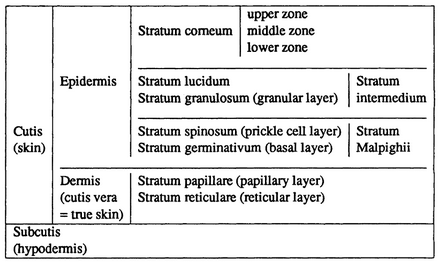
\includegraphics[width=0.8\textwidth]{images/skinLayers.png}
\caption{The Layers of the skin.The zonal layering is not so distinct in every skin region. Note that the stratum lucidum is only clearly recognizable on the palmar and plantar skin areas.\citep{HANDBOOKPP}}
\label{layerTab}
\end{figure}

%epidermis
The epidermis, on its own, can be divided into five different layers and lies on the surface of the skin. It consists of epithelial tissue, which is built in the lowest layer, the stratum germinativum. The main part of the produced cells are keratinocytes, which are able to store keratin and therefore become horny over time. The keratinocytes migrate to the surface of the skin, causing the epidermis to become more horny when approaching the surface. The outer layer is called the stratum corneum, originating from the fully keratinized state of its cells.
On their way to the surface the keratinocytes undergo a number of specific changes in form and areal  distribution, which in part are used to define the different epidermal layers. Also the cells become less tightly packed, compared to the deeper layers, causing the epidermis to become dryer towards the surface. A fact that greatly influences the electrical properties of the epidermis and therefore the  electrodermal activity. The stratum corneum is especially thick in the palmar and plantar regions of the body. Reaching a thickness of approximately 1 $mm$, it is almost 20 times thicker than its overall average of 50 $\mu m$.
%dermis
The dermis, which is also referred to as the corium, lies directly beneath the epidermis. Although it is much thicker than the epidermis it is only composed of two different dermal layers, the stratum papillare and the stratum reticulare, which are distinguishable by their density and the arrangement of their collagen fibers. The epidermal dermal junction, which is the transition area between the epidermis and dermis, resembles interlocking hands, forming a close connection between the two.
The dermal layer, closest to the epidermis is called the papillary stratum.
 
%recap link to sweat glands
The figure \ref{layerImg} shows an example of a typical profile of glabrous (hairless) skin. This specific form of skin can be found on the palms of the hands and the soles of the feet. Areas, both of which, are frequently mechanically stressed and differ greatly from the rest of the body.

\begin{figure}[ht]
\centering
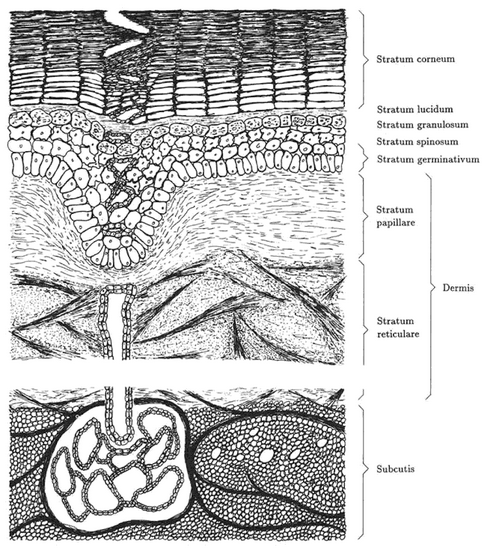
\includegraphics[width=0.7\textwidth]{images/skinGlabrous.png}
\caption{A cross-section of the layered construction of the glabrous human skin. An eccrine\citep{HANDBOOKPP}}
\label{layerImg}
\end{figure}




\begin{figure}[ht]
\centering
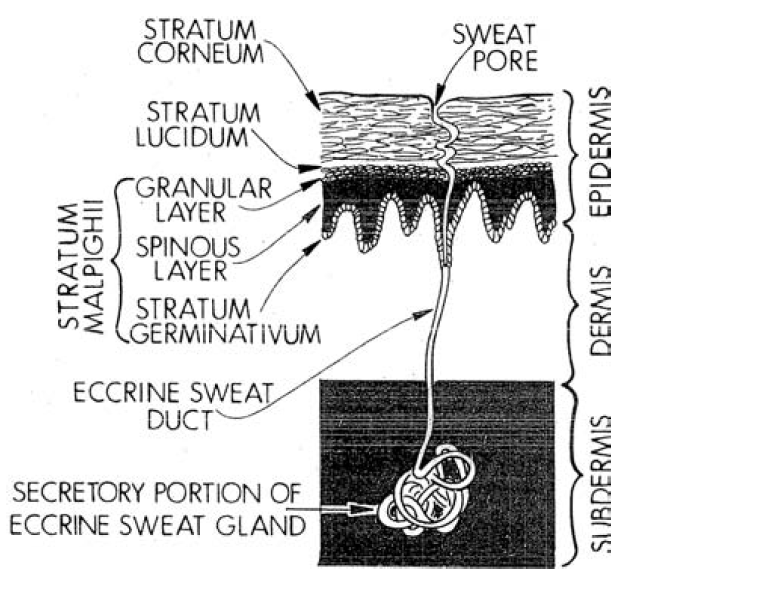
\includegraphics[width=0.7\textwidth]{images/skinAnatomy.png}
\caption{Anatomy of the eccrine sweat gland in various layers of glabrous skin.(Adapted from Hassett, 1978)\citep{HANDBOOKPP}}
\label{layerImg}
\end{figure}




% -functions of the skin -heat regulation -sweat gland activity 

\subsection{Exposure Therapy}
%what is exposure therapy?\\ 
%when is it used? \\
%how is it done?\\
%what is needed for it to be successful? \\
%how effective is it?\\
%
\section{General}
\subsection{State of the Art}
\subsection{Recent Advances in Research}
\section{Problem Analysis and Goals}
%- analyze the problem with current models of exposure therapy
%- show that my approach is different and how
%- why my approach is better and makes sense
%- goal is a safe and effective therapy option for acrophobia
%
%
